% /*
%  * ----------------------------------------------------------------------------
%  * "THE BEER-WARE LICENSE" (Revision 42):
%  * <michi.wieland@hotmail.com> wrote this file. As long as you retain this notice you
%  * can do whatever you want with this stuff. If we meet some day, and you think
%  * this stuff is worth it, you can buy me a beer in return. Michael Wieland
%  * ----------------------------------------------------------------------------
%  */

\documentclass[
a4paper,
oneside,
10pt,
fleqn,
headsepline,
toc=listofnumbered, 
bibliography=totocnumbered]{scrartcl}

% deutsche Trennmuster etc.
\usepackage[T1]{fontenc}
\usepackage[utf8]{inputenc}
\usepackage[english, ngerman]{babel} % \selectlanguage{english} if  needed
\usepackage{lmodern} % use modern latin fonts

% Custom commands
\newcommand{\AUTHOR}{Michael Wieland}
\newcommand{\INSTITUTE}{Hochschule für Technik Rapperswil}
\newcommand{\GITHUB}{https://github.com/michiwieland/hsr-zusammenfassungen}
\newcommand{\LICENSEURL}{https://en.wikipedia.org/wiki/Beerware}
\newcommand{\LICENSE}{
"THE BEER-WARE LICENSE" (Revision 42):
<michi.wieland@hotmail.com> wrote this file. As long as you retain this notice you
can do whatever you want with this stuff. If we meet some day, and you think
this stuff is worth it, you can buy me a beer in return. Michael Wieland	
}

% Jede Überschrift 1 auf neuer Seite
\let\stdsection\section
\renewcommand\section{\clearpage\stdsection}

% Multiple Authors
\usepackage{authblk}

% Include external pdf
\usepackage{pdfpages}

% Layout / Seitenränder
\usepackage{geometry}

% Inhaltsverzeichnis
\usepackage{makeidx} 
\makeindex

\usepackage{url}
\usepackage[pdfborder={0 0 0}]{hyperref}
\usepackage[all]{hypcap}
\usepackage{hyperxmp} % for license metadata

% Glossar und Abkürzungsverzeichnis
\usepackage[acronym,toc,nopostdot]{glossaries}
\glossarystyle{altlist}
\usepackage{xparse}
\DeclareDocumentCommand{\newdualentry}{ O{} O{} m m m m } {
	\newglossaryentry{gls-#3}{
		name={#4 : #5},
		text={#5\glsadd{#3}},
		description={#6},
		#1
	}
	\makeglossaries
	\newacronym[see={[Siehe:]{gls-#3}},#2]{#3}{#4}{#5\glsadd{gls-#3}}
}
\makeglossaries

% Mathematik
\usepackage{amsmath}
\usepackage{amssymb}
\usepackage{amsfonts}
\usepackage{enumitem}

% Images
\usepackage{graphicx}
\graphicspath{{images/}} % default paths

% Boxes
\usepackage{fancybox}

%Tables
\usepackage{tabu}
\usepackage{booktabs} % toprule, midrule, bottomrule
\usepackage{array} % for matrix tables

% Multi Columns
\usepackage{multicol}

% Header and footer
\usepackage{scrlayer-scrpage}
\setkomafont{pagehead}{\normalfont}
\setkomafont{pagefoot}{\normalfont}
\automark*{section}
\clearpairofpagestyles
\ihead{\headmark}
\ohead{\AUTHOR}
\cfoot{\pagemark}

% Pseudocode
\usepackage{algorithmic}
\usepackage[linesnumbered,ruled]{algorithm2e}

% Code Listings
\usepackage{listings}
\usepackage{color}
\usepackage{beramono}

\definecolor{bluekeywords}{rgb}{0,0,1}
\definecolor{greencomments}{rgb}{0,0.5,0}
\definecolor{redstrings}{rgb}{0.64,0.08,0.08}
\definecolor{xmlcomments}{rgb}{0.5,0.5,0.5}
\definecolor{types}{rgb}{0.17,0.57,0.68}

\lstdefinestyle{visual-studio-style}{
	language=[Sharp]C,
	columns=flexible,
	showstringspaces=false,
	basicstyle=\footnotesize\ttfamily, 
	commentstyle=\color{greencomments},
	morekeywords={partial, var, value, get, set},
	keywordstyle=\bfseries\color{bluekeywords},
	stringstyle=\color{redstrings},
	breaklines=true,
	breakatwhitespace=true,
	tabsize=4,
	numbers=left,
	numberstyle=\tiny\color{black},
	frame=lines,
	showspaces=false,
	showtabs=false,
	escapeinside={£}{£},
}

\definecolor{DarkPurple}{rgb}{0.4, 0.1, 0.4}
\definecolor{DarkCyan}{rgb}{0.0, 0.5, 0.4}
\definecolor{LightLime}{rgb}{0.3, 0.5, 0.4}
\definecolor{Blue}{rgb}{0.0, 0.0, 1.0}

\lstdefinestyle{cevelop-style}{
	language=C++,  
	columns=flexible,
	showstringspaces=false,     
	basicstyle=\footnotesize\ttfamily, 
	keywordstyle=\bfseries\color{DarkPurple},
	commentstyle=\color{LightLime},
	stringstyle=\color{Blue}, 
	escapeinside={£}{£}, % latex scope within code      
	breaklines=true,
	breakatwhitespace=true,
	showspaces=false,
	showtabs=false,
	tabsize=4,
	morekeywords={include,ifndef,define},
	numbers=left,
	numberstyle=\tiny\color{black},
	frame=lines,
}

\lstdefinestyle{eclipse-style}{
	language=Java,  
	columns=flexible,
	showstringspaces=false,     
	basicstyle=\footnotesize\ttfamily, 
	keywordstyle=\bfseries\color{DarkPurple},
	commentstyle=\color{LightLime},
	stringstyle=\color{Blue}, 
	escapeinside={£}{£}, % latex scope within code      
	breaklines=true,
	breakatwhitespace=true,
	showspaces=false,
	showtabs=false,
	tabsize=4,
	morekeywords={length},
	numbers=left,
	numberstyle=\tiny\color{black},
	frame=lines,
}
\lstset{style=eclipse-style}



% Theorems \begin{mytheo}{title}{label}
\usepackage{tcolorbox}
\tcbuselibrary{theorems}
\newtcbtheorem[number within=section]{definiton}{Definition}%
{fonttitle=\bfseries}{def}
\newtcbtheorem[number within=section]{remember}{Merke}%
{fonttitle=\bfseries}{rem}
\newtcbtheorem[number within=section]{hint}{Hinweis}%
{fonttitle=\bfseries}{hnt}

% Dokumentinformationen
\newcommand{\SUBJECT}{Zusammenfassung}
\newcommand{\TITLE}{Algorithmen und Datenstrukturen 1}

% pdf metadata
\hypersetup{
	pdfauthor={\AUTHOR},
	pdftitle={\SUBJECT \TITLE},
	pdfcopyright={\LICENSE},
	pdflicenseurl={\LICENSEURL}
}

\begin{document}
	
% Front page
\title{\TITLE}
\subject{\SUBJECT}
\author{\AUTHOR}
\affil{\INSTITUTE}
\date{\today}
\maketitle

\vfill

% Participate
\paragraph{Mitmachen} \hfill \\
Falls Du an diesem Dokument mitarbeiten willst, kannst Du das Dokument
auf GitHub unter \url{\GITHUB} forken.

% Licence
\paragraph{Lizenz} \hfill \\
\LICENSE

% Table of contents
\tableofcontents


% Glossar and acronyms (if included \loadglsentries{glossar})
\printglossary[type=\acronymtype]
\printglossary
\glsaddall


\section{Generelles}
\begin{description}
	\item[ADT: Abstract Data Type] \hfill \\
	Ein abstrakter Datentyp beschreibt eine Datenstruktur generell, sodass diese in einer beliebigen Sprache umgesetzt werden kann.
	\item[Sentinel Objekte] \hfill \\
	Sind Wächter Objekte die an den Enden von z.B einer Linked List vorkommen. Ein Sentinel ist also ein Terminator einer Sequenz (Header, Trailer)
	\item[NIL] Not in List
	\item[Default Initialisierung (Java)] \hfill
	\begin{itemize}
		\item Primitive Datentypen: 0
		\item Boolsche Datentypen: false
		\item Objekte (auch Strings): null 
	\end{itemize}
	\item[String Konkatinierung] \hfill \\
	Für das Zusammensetzen von String sollte immer ein StringBuilder verwendet werden. Insbesondere bei grosser Anzahl von Teilstrings ist der Zeitunterschied enorm.
\end{description}

\subsection{Comparator}
\begin{itemize}
	\item Die beiden Objekte a und b müssen das Interface Comparable implementieren. Ansonsten soll eine Exception geworfen werden
	\item compare(a, b)
	\begin{itemize}
		\item falls a < b $\Rightarrow$ negativ Wert
		\item falls a = b $\Rightarrow$ 0
		\item falls a > b $\Rightarrow$ positiver Wert
	\end{itemize}
\end{itemize}

\subsection{Switch Case}
Folgende Datentypen können in einer Switch Anweisung verwendet werden
\begin{itemize}
	\item byte, short, char, int
	\item Enumerations
	\item String, Character, Byte, Short, Integer
\end{itemize}
\begin{lstlisting}
switch(n) {
	case 1: n + 1; break; 
	case 2: n + 2; 
	// also executed for case 2, because of missing break;
	case 2: n + 3; 
}
\end{lstlisting}

\section{Mathematische Grundlagen}
\subsection{Allgemeine Summenformel}
\[
\sum\limits_{i=1}^{n} a_i = \frac{n(a_n + a_1)}{2} = \frac{n(n+1)}{2}
\]

\subsection{Geometrische Reihe}
Muss bei Exponentiellem Wachstum verwendet werden.
\[
\sum\limits_{i=0}^{n} a^i = \frac{a^{n+1} - 1}{a - 1}
\]

\subsection{Fakultät}
\[
n! = 1 \cdot 2 \cdot 3 \cdot ... \cdot n = \prod_{k=1}^n k
\]
\[
n! \cdot (n + 1) = (n+1)!
\]
wobei
\[
	0! = 1
\]

\subsection{Beispiel: Arithmetische Folgen}
Bestimmen Sie da n-te Glied ($a_n$) der Folge 1,5,9,13,17:
\paragraph{Rekursiv:} $a_1 = 1$ und $a_n= a_{n-1} + 4$
\paragraph{Iterativ:} $a_1 + \sum\limits_{i=2}^{n}4$
\paragraph{Explizit:} $a_1 + incr \cdot(n-1) = 1+ 4(n-1) = 4n - 3$

\subsection{Beispiel: Summenformelbeweis}
\[
	\sum_{i=n}^{2n-1} \frac{1}{i} = \sum_{i=n}^{2n-1} \frac{(-1)^{i+1}}{i}
\]

\subsubsection{Verankerung n=1}
linke Seite = rechte Seite?
\begin{align}
	\begin{split}
	\sum_{i=1}^{1} \frac{1}{1} &= \sum_{i=1}^{1} \frac{(-1)^{1+1}}{1} \\
	1 &= 1 \Rightarrow \text{erfüllt}
	\end{split}
\end{align}

\subsubsection{Induktionsschritt n = n + 1} \hfill \\
\paragraph{linke Seite:}
\begin{align}
	\begin{split}
	\sum_{n}^{2n-1} \Rightarrow \sum_{n+1}^{2n+1} \\
	\end{split}
\end{align}
Die beiden Summenformeln ausschreiben und Unterschiede markieren. 
\begin{align}
	\begin{split}
			\frac{1}{n} &+ \frac{1}{n+1} + \frac{1}{n+2} + ... + \frac{1}{2n-2} + \frac{1}{2n-1} \\
			&\frac{1}{n+1} + \frac{1}{n+2} + ....................... + \frac{1}{2n-1} + \frac{1}{2n} + \frac{1}{2n+1}
	\end{split}
\end{align}

Unterschiede an bestehendes Anhängen
\begin{align}
	\begin{split}
		\sum_{n}^{2n-1} \frac{1}{i} - (\frac{1}{n}) + (\frac{1}{2n}) + (\frac{1}{2n+1})
	\end{split}
\end{align}

\paragraph{rechte Seite:}
\begin{align}
	\begin{split}
		\sum_{1}^{2n-1} \Rightarrow \sum_{1}^{2n+1} \\
	\end{split}
\end{align}
Die beiden Summenformeln ausschreiben und Unterschiede markieren. 
\begin{align}
	\begin{split}
		\frac{(-1)^{2}}{1} + \frac{(-1)^{3}}{2} + 	\frac{(-1)^{4}}{3} + ... + \frac{(-1)^{2n-1}}{2n-2} &+\frac{(-1)^{2n}}{2n-1} \\
		\frac{(-1)^{2}}{1} + \frac{(-1)^{3}}{2} + 	\frac{(-1)^{4}}{3} + ....................... &+ \frac{(-1)^{2n}}{2n - 1} + \frac{(-1)^{2n+1}}{2n} + 	\frac{(-1)^{2n + 2}}{2n+1}
	\end{split}
\end{align}

Unterschiede an bestehendes Anhängen
\begin{align}
	\begin{split}
		\sum_{1}^{2n-1} \frac{(-1)^{i+1}}{i} + (\frac{(-1)^{2n+1}}{2n}) + (\frac{(-1)^{2n + 2}}{2n+1})
	\end{split}
\end{align}

\paragraph{Zusammenführen} \hfill \\
Nun können die Summenformeln weggelassen werden, da diese gemäss Induktionsbehauptung äquivalent sind.
\begin{align}
	\begin{split}
	\frac{1}{2n} + \frac{1}{2n+1} - \frac{1}{n} &= \frac{(-1)^{2n+1}}{2n} + \frac{(-1)^{2n + 2}}{2n+1} \\
	\frac{1}{2n} + \frac{1}{2n+1} - \frac{1}{n} &= \frac{\overbrace{(-1)^{2n+1}}^{-1}}{2n} + \frac{\overbrace{(-1)^{2n + 2}}^{1}}{2n+1} \\
	\frac{1}{2n} - \frac{1}{n} &= \frac{-1}{2n} \\
	\frac{1}{2n} + \frac{1}{2n}  - \frac{1}{n} &= 0 \\
	\frac{2}{2n} &= \frac{1}{n} \\
	\frac{1}{n} &= \frac{1}{n}
	\end{split}
\end{align}

\subsection{Beispiel: Rekursive Abschätzung}
Gegeben sei folgende rekursive Abschätzung des Zeitverhaltens eines Algorithmus:
\begin{align*}
\begin{split}
	T(n) &= 16 \cdot T(\frac{n}{4}) - 33 \cdot n + 15 \\
	T(1) &= S \text{ (Startwert)} = 10
\end{split}
\end{align*}
\paragraph{Fragestellung:} Ist $T(n) \in \mathcal{O}(n)$ oder $T(n) \in \mathcal{O}(n^2)$?

\paragraph{Lösungs-Ansatz} $T(n) = a\cdot n^2 + b\cdot n + c$

\paragraph{Auflösen von Variablen}
\begin{align}
\begin{split}
T(\frac{n}{4}) \Rightarrow T(n) &= a\cdot n^2 + b\cdot n + c \\
T(\frac{n}{4}) &= \frac{a\cdot n^2}{16} + \frac{b\cdot n}{4} + c
\end{split}
\end{align}

\paragraph{Einsetzen und Vereinfachen}
Nun kann $T(\frac{n}{4})$ in die rekursive Laufzeitabschätzung eingesetzt, und mit der beispielhaften Laufzeit von $\mathcal{O}(n^2)$ gleichsetzt werden.
\begin{align}
\begin{split}
	16 \cdot \overbrace{(\frac{a \cdot n^2}{16} + \frac{b \cdot n}{4} + c)}^{T(\frac{n}{4})} - 33 \cdot n + 15 &= \overbrace{a \cdot n^2 + bn + c}^{\mathcal{O}(n^2)} \\
	\Leftrightarrow a \cdot n^2 + 4bn + 16c - 33n + 15 &= a \cdot n^2 + bn + c
\end{split}
\end{align}

\paragraph{Behandlung der quadratischen Teile $n^2$}
\begin{align}
\begin{split}
	a \cdot n^2 &= a \cdot n^2 \\
	a &= a
\end{split}
\end{align}

\paragraph{Behandlung der linearen Teile n}
\begin{align}
\begin{split}
	4bn - 33n &= bn \\
	4b - 33 &= b \\
	-33 &= -3b \\
	b &= 11
\end{split}
\end{align}

\paragraph{Behandlung der konstanten Teile c}
\begin{align}
\begin{split}
	16c + 15 &= c \\
	15 &= -15c \\
	c &= -1
\end{split}
\end{align}

\paragraph{Laufzeit angeben}
Es sei der Startwert $T(1) = 10$ gegeben:
\begin{align}
\begin{split}
10 &= n^2\cdot a + n \cdot b + c \\
10 &= 1\cdot a + 1 \cdot 11 - 1 \\
a &= 0 \Rightarrow n^2 \text{ Teile sind Null und daher ist die Laufzeit = } \underline{\underline{\mathcal{O}(n)}}
\end{split}
\end{align}

\section{Beweisen}
Der Beweis durch vollständige Induktion sei folgend anhand einem Beispiel erklärt

\[
\sum\limits_{k=1}^{n} \frac{1}{k(k+1)} = \frac{n}{n + 1} \text{ wobei } n \geq 1
\]

\subsection{Induktionsverankerung (n = 1)}
Ist die linke Seite gleich der rechten Seite?
\begin{enumerate}
	\item Linke Seite: $\frac{1}{1(1+1)} = \frac{1}{2}$
	
	\item Rechte Seite: $\frac{1}{2}$
\end{enumerate}
Die Induktionsverankerung ist somit erfüllt.

\subsection{Induktionsschritt (n = n + 1)}
\subsubsection{Induktionsannahme}
Unsere Annahme ist, dass die Induktionsverankerung für n gilt. Man schreibt noch einmal die Verankerung hin.
\[
\sum\limits_{k=1}^{n} \frac{1}{k(k+1)} = \frac{n}{n + 1}
\]

\subsubsection{Induktionsbehauptung}
Somit muss sie die Annahme auch für $n = n + 1$ gelten. Man ersetze alle $n$ mit $n + 1$
\[
\sum\limits_{k=1}^{n + 1} \frac{1}{k(k+1)} = \frac{n + 1}{n + 2}
\]

\subsubsection{Induktionsbeweis}
\[
\underbrace{\frac{n}{n + 1}}_{\text{rechte Seite der Annahme}} + \underbrace{\frac{1}{(n+1)(n+2)}}_{\text{k = n+1 aus Annahme}} = \underbrace{\frac{n+1}{n+2}}_{\text{rechte Seite der Behauptung}}
\]

\[ \Leftrightarrow n(n+2) + 1 = (n+1)^2 \]
\[ \Leftrightarrow n^2 + 2n + 1 = n^2 + 2n +1 \]
\[ \rightarrow \text{Erfüllt, quod erat demonstrandum} \]


\section{Landau-Symbole}
\subsection{Big Oh Notation $\mathcal{O}(x)$}
\begin{itemize}
	\item Bei der Big Oh Notation konzentriert man sich immer auf den Worst Case. 
	\item Die Big Oh Notation lässt sich die Laufzeit und Speicherverbrauch eines Algorithmus beschreiben
	\item Dabei wird immer ein konkreter Fall angeschaut. (z.B die Laufzeit einer Schleife unter Bedingung i > 1) 
	\item f(n) ist $\mathcal{O}$(g(n)) falls f(n) asymptotisch kleiner oder gleich wie g(n) ist
\end{itemize}

\subsubsection{Vorgehen}
\begin{enumerate}
	\item primitive Operationen Zähle, rsp. wie oft eine Anweisung ausgeführt wird.
	\item Konstante Faktoren können weggelassen werden
	\item Gibt es mehrere Potenzen ($n^2$, $n^5$) gilt nur die höchste. Alle anderen können ebenfalls weggelassen werden.
	\item $\mathcal{O}$(x) aufschreiben. z.B $\mathcal{O}$($n^2$) oder $\mathcal{O}(n)$
\end{enumerate}

\subsection{Big Omega Notation $\Omega(x)$}
\begin{itemize}
	\item f(n) ist $\Omega$(g(n)) falls f(n) asymptotisch grösser oder gleich wie g(n) ist
\end{itemize}

\subsection{Big Theta Notation $\Theta(x)$}
\begin{itemize}
	\item f(n) ist $\Theta$(g(n)) falls f(n) asymptotisch gleich wie g(n) ist
\end{itemize}


\begin{figure}[h!]
\centering
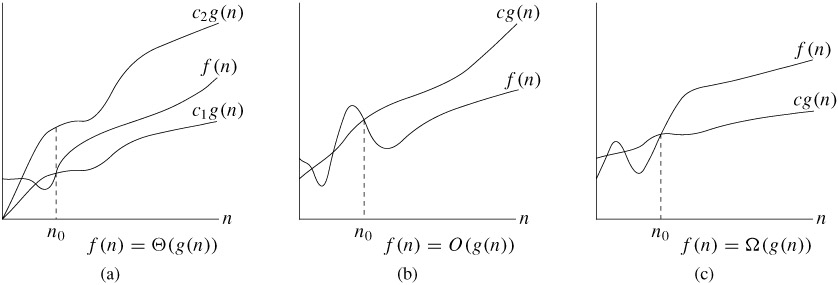
\includegraphics[width=0.9\linewidth]{images/big_oh_omega_theta}
\caption{Big Theta / Big Oh / Big Omega}
\end{figure}


\section{Analyse von Algorithmen}
\begin{description}
	\item[Algorithmus] \hfill \\
	Ein Algorithmus ist ein Schritt für Schritt Vorgehen zum Lösen eines Problems mit endlichem Zeitaufwand.
\end{description}

\subsection{Laufzeiten}
\begin{enumerate}
	\item $\mathcal{O}(1)$ = konstant 
	\item $\mathcal{O}$(log(n)) = logarithmisch
	\item $\mathcal{O}(n)$ = linear
	\item $\mathcal{O}$(n log(n)) = n-Log-n
	\item $\mathcal{O}$($n^2$) = Quadratisch
	\item $\mathcal{O}$($n^3$) = Qubisch
	\item $\mathcal{O}$($2^n$) = Exponentiell
	\item $\mathcal{O}$($n!$) = Fakultät
\end{enumerate}

\begin{figure}[h]
	\centering
	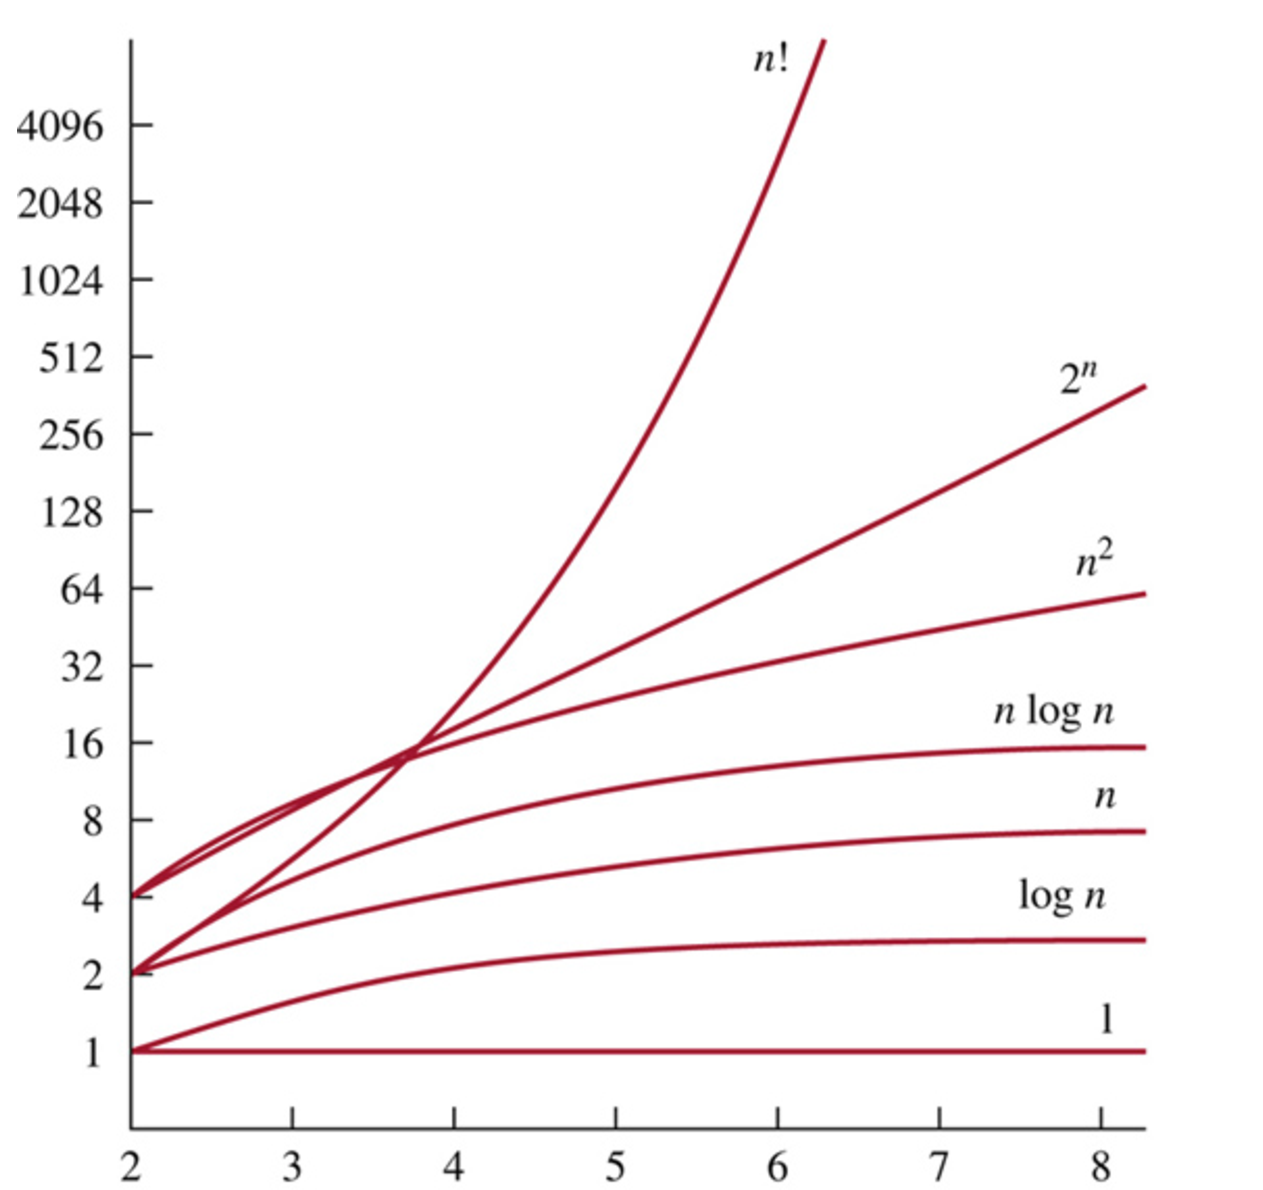
\includegraphics[width=0.4\linewidth]{images/laufzeiten}
	\caption{Laufzeiten}
\end{figure}

\section{UML: Unified Modeling Language}
\begin{description}
	\item[Aggregation und Komposition] \hfill \\
	Beide sind ''Ist-Teil-von-Ganzem'' Beziehung, wobei die Komposition stärker bindet. Wird bei der Komposition der Parent gelöscht, müssen auch alle Childs gelöst werden.
\end{description}
\begin{figure}[h]
	\centering
	\begin{minipage}[t]{0.4\textwidth}
		\centering
		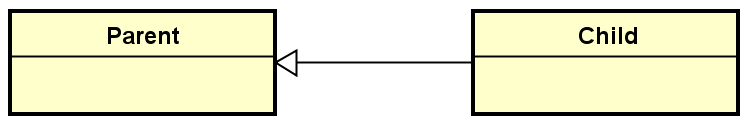
\includegraphics[width=\textwidth]{images/generalisierung}
		\caption{Generalisierung}
	\end{minipage}
	\begin{minipage}[t]{0.4\textwidth}
		\centering
		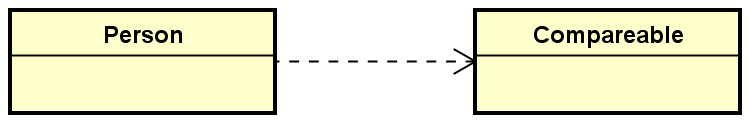
\includegraphics[width=\textwidth]{images/implements}
		\caption{Implementierung / Dependency}
	\end{minipage}
\end{figure}
\begin{figure}[ht!]
	\centering
	\begin{minipage}[t]{0.4\textwidth}
		\centering
		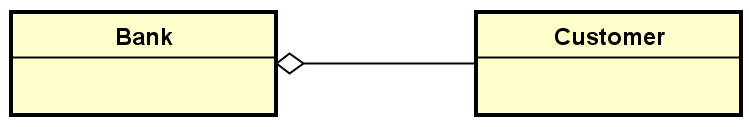
\includegraphics[width=\textwidth]{images/aggregation}
		\caption{Aggregation}
	\end{minipage}
	\begin{minipage}[t]{0.4\textwidth}
		\centering
		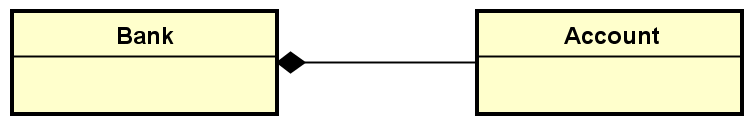
\includegraphics[width=\textwidth]{images/composition}
		\caption{Komposition}
	\end{minipage}
\end{figure}
\section{Design Pattern}
\subsection{Adapter Pattern}
Das Entwurfsmuster findet in erster Linie Anwendung, wenn eine existierende Klasse verwendet werden soll, deren Schnittstelle nicht der benötigten Schnittstelle entspricht. Adapter ermöglichen die Zusammenarbeit von Klassen, die ohne nicht zusammenarbeiten könnten, weil sie inkompatible Schnittstellen haben. Es gibt zwei Varianten von Adaptern:

\subsubsection{Objektadapter}
\begin{itemize}
	\item Auch als Wrapper bekannt
	\item Verwendet Komposition, welche zur Laufzeit hinzugefügt wird. Die Adapter Klasse besitzt also eine Instanzvariable vom Typ des Adaptee
	\item Kapselt besser, da die Methoden des Adaptee nicht sichtbar sind
	\item Alle Methoden die der Adapter zur Verfügung soll, müssen im Target Interface implementiert sein.
	\item Wird verwendet wenn man dem Client nur Methoden mit abgeänderter Adaptee Funktionalität zur Verfügung stellen möchte. Die restliche Adaptee Funktionalität soll aber versteckt bleiben.
	\item Der Objektadapter wird wie folgt verwendet: 
	\begin{lstlisting}
		public class Client {
			// Adapter implements Target
			private Target myAdapter = new Adapter();
			
			public Client() {
				myAdapter.request();
			}
		}
	\end{lstlisting}
\end{itemize}

\begin{figure}[h]
	\centering
	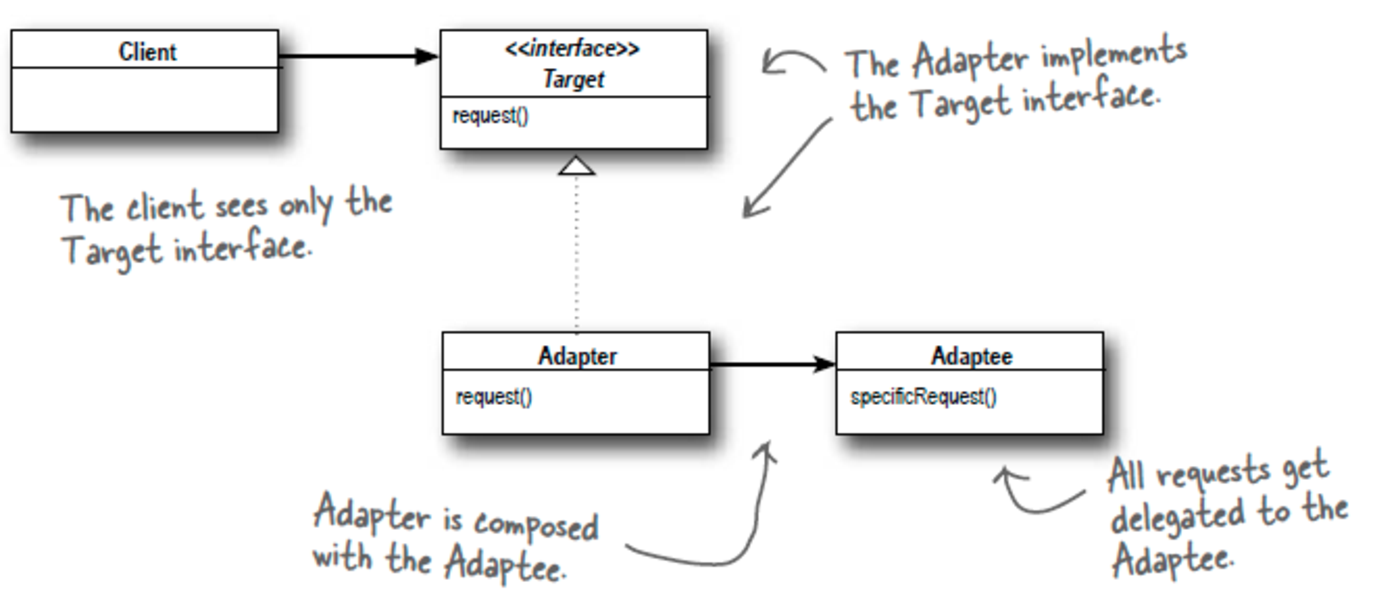
\includegraphics[width=1\linewidth]{images/object_adapter_uml}
	\caption{Objekt Adapter Pattern}
\end{figure}


\subsubsection{Klassenadapter}
\begin{itemize}
	\item Verwendet Mehrfachvererbung welche bereits zur Compilezeit fixiert ist. Unter Java muss ein Interface und einer abstrakte Klasse verwendet werden, da Java keine Mehrfachvererbung unterstützt.
	\item Trägt die Methoden des Adaptess nach aussen
	\item Wird verwendet wenn eine zusätzliche Methode implementiert werden soll und man aber immer noch auf die  Methoden des Adaptee zugreifen soll.
	\item Der Klassenadapter wird wie folgt verwendet: 
	\begin{lstlisting}
	public class Client {
		// Adapter extends Adaptee implements Target
		private Target myAdapter = new Adapter();
	
		public Client() {
			myAdapter.request();
			myAdapter.adapteeMethod();
		}
	}
	\end{lstlisting}
\end{itemize}
\begin{figure}[h]
	\centering
	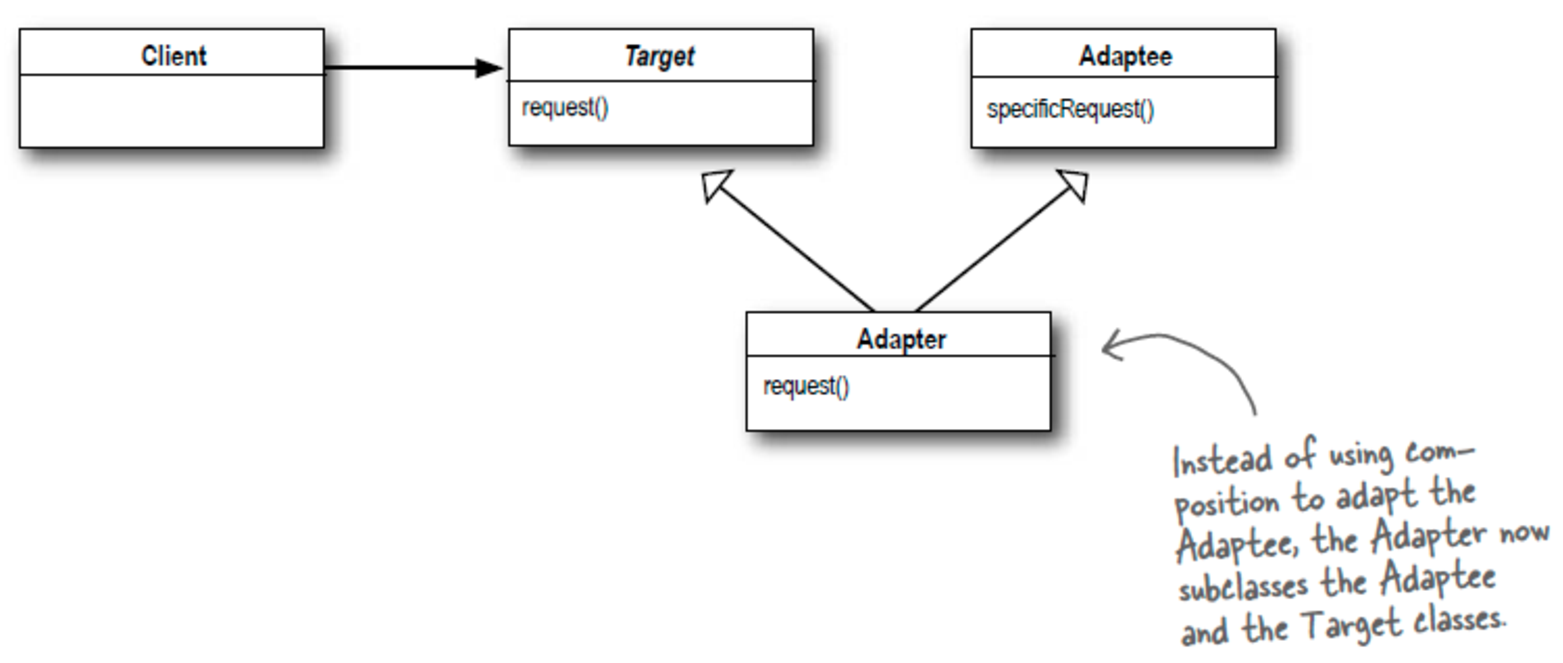
\includegraphics[width=0.9\linewidth]{images/class_adapter_uml.pdf}
	\caption{Klassen Adapter Pattern}
\end{figure}

\subsection{Template Method Pattern}
\begin{itemize}
	\item Die gemeinsamen Teile werden in einer abstrakten Klasse implementiert und in den Subklassen bei Bedarf verfeinert.
	\item Die abstrakte Klasse besteht aus unveränderlichen Methoden welche zusätzlich abstrakte Methoden (Hooks) aufruft, welche in der Subklasse überschrieben werden müssen.
	\item Das Pattern verwendet das Hollywood Prinzip: ''Don't call us, we call you''
	\begin{lstlisting}
	public abstract class Game {
		abstract void initialize();
		abstract void startPlay();
		abstract void endPlay();
		
		//template method
		public final void play(){
			
			//initialize the game
			initialize();
			
			//start game
			startPlay();
			
			//end game
			endPlay();
		}
	}
	
	public class Football extends Game {
		@Override
		void endPlay() {
			System.out.println("Football Game Finished!");
		}
		
		@Override
		void initialize() {
			System.out.println("Football Game Initialized! Start playing.");
		}
		
		@Override
		void startPlay() {
			System.out.println("Football Game Started. Enjoy the game!");
		}
	}
	\end{lstlisting}
\end{itemize}
\begin{figure}[h]
	\centering
	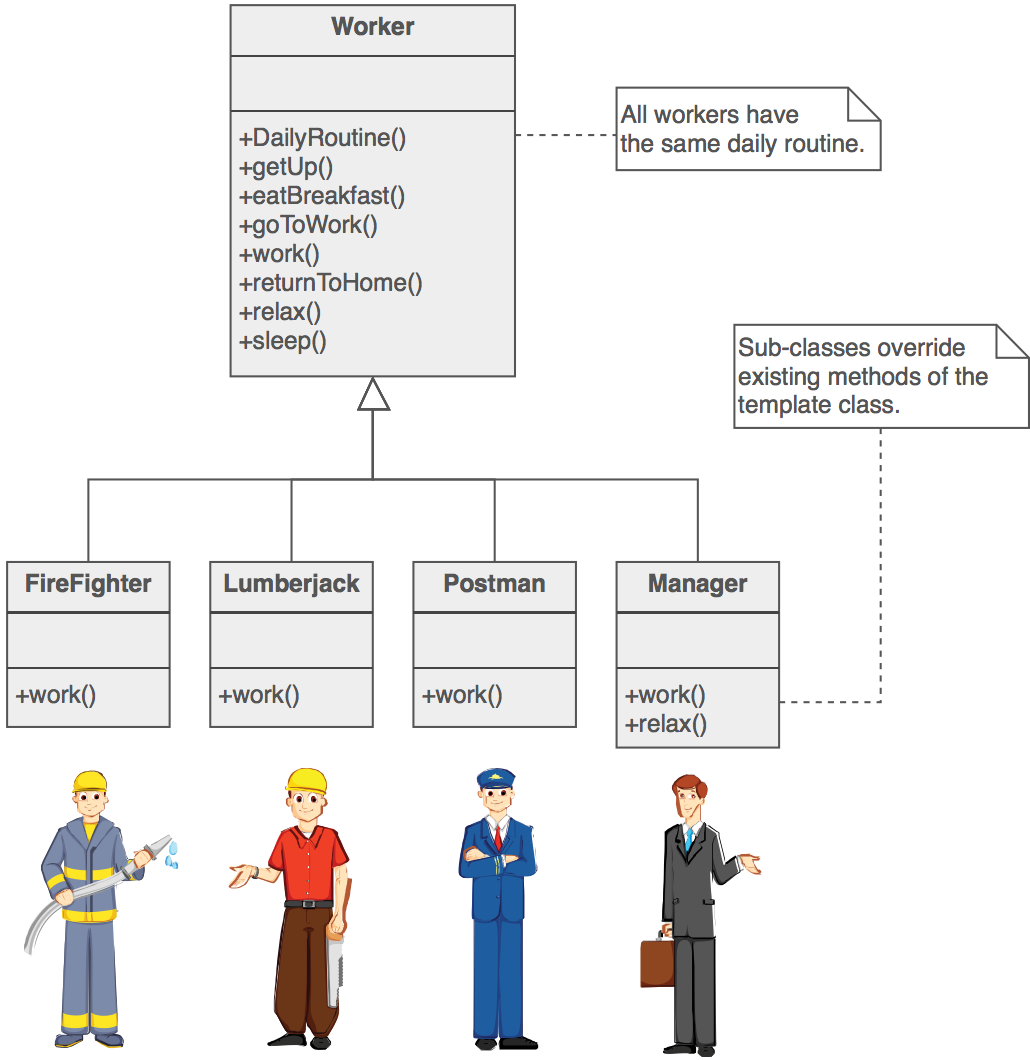
\includegraphics[width=0.6\linewidth]{images/template_methode_pattern}
	\caption{Template Method Pattern}
\end{figure}

\section{Rekursion}
\subsection{Rekursion vs Iteration}
\begin{itemize}
	\item Iteration brauch kaum Speicher. Die Iterationsvariablen müssen einmal alloziert und können anschliessend nur noch inkrementiert werden.
	\item Rekursion muss immer wieder einen neuen Stack anlegen. Es droht die Gefahr eines Stack Overflows!
	\item Iteration ist schneller
	\item Alle Rekursionen können als Iteration ausgedrückt werden.
	\item Es gibt aber Probleme die nur sehr schwer iterativ gelöst werden können. 
\end{itemize}

\subsection{Lineare Rekursion}
Eine lineare rekursive Methode ruft sich solange auf bis sie den BaseCase / Abbruchkriterium erreicht. Die Rekursion legt die Zwischenresultate auf den Stack und rechnet diese nach dem Ankommen beim Base Case rückwärts zusammen.

\subsubsection{Fibonacci Folge}
\begin{lstlisting}
// Return fibonacci sequence (0 1 1 2 3 5 8 13 ...)
public static int fibonacci(int number){
	// Base case
	if(number <= 1){
		return number;
	} 
	return fibonacci(number-1) + fibonacci(number -2);
}
\end{lstlisting}

\subsubsection{Divide \& Conquer}
\begin{enumerate}
	\item Ein grosses Problem in mehrere Teile zerlegen bis ein kleines Problem trivial zu lösen ist (z.B Binär sortieren)
	\item Base Case ist wenn nur noch ein Element vorig ist
	\item Dieser Lösungsansatz wird für viele bekannte Algorithmen verwendet. So zum Beispiel Fibonacci, Quicksort, Euklid und Tower of Hanoi.
\end{enumerate}

\subsubsection{Tail Rekursion / Endrekursion}
Bei einer Tail Rekursion muss die letzte Operation ein rekursiver Aufruf sein. Bei einer ''normalen'' Rekursion steigt der Speicherplatzverbrauch linear mit der Rekursionstiefe. Da bei Tail Rekursionen aber das Resultat beim erreichen des Base Cases vorhanden ist, muss nur Speicherplatz für die Übergabe der Methodenparameter reserviert werden. Der restliche Speicherplatz kann wieder freigegeben werden.  Somit ist der Speicherplatzverbrauch bei einer Tail Rekursion unabhängig von der Rekursionstiefe. Compiler wandlen Endrekursionen im Rahmen eines Optimierungsschrittes sogar direkt in die iterative Form um.

\subsubsection{Rekursives Summieren}
\begin{lstlisting}
int sum(int i, int sum) { 
	if(i == 0) {
		return sum; 
	} 
	return sum(i-1, i + sum);  
}
\end{lstlisting}



\subsection{Binäre Rekursion}
Bei der binären Rekursion existieren zwei rekursive Aufrufe in allen nicht-terminalen (kein Base Case) Aufrufen. 

\subsubsection{Tower of Hanoi}
\[
	Anzahl_{moves} = 2^n - 1
\]
wobei
\begin{itemize}[label=]
	\item[n] Anzahl Disks
\end{itemize}

\begin{lstlisting}
// Tower of Hanoi
public class TowerOfHanoi {
	public static void main(String[] args) {
		int amountOfDisks = 3;
		doTowers(amountOfDisks, 'A', 'B', 'C');
	}
	
	public void solve(int n, String start, String auxiliary, String end) {
		 if (n == 1) {
			 System.out.println("Disk-" + n + " from " +  start + " to " + end);
		 } else {
			 solve(n - 1, start, end, auxiliary);
			 System.out.println("Disk-" + n + " from " +  start + " to " + end);
			 solve(n - 1, auxiliary, start, end);
		 }
	 }
	 
}
\end{lstlisting}


\section{Arrays}
\begin{itemize}
	\item Random Access: Man kann auf jedes beliebige Element mit $\mathcal{O}(1)$ zugreifen
	\item Keine dynamische Grösse
	\item In Java speichern Arrays von Objekten nur die Referenz auf das Objekt und nicht das Objekt selbst (Ausnahme: primitive Datentypen)
	\item Nützliche Array Methoden:
	\begin{lstlisting}
	// Vergleichen
	Arrays.equals(object[] a1, object[] a2);
	
	// Sortieren
	Arrays.sort(object[] a1);
	
	// Umkopieren
	System.arraycopy(Object src, int srcPos, Object dest, int destPos, int length)
	\end{lstlisting}
\end{itemize}

\begin{figure}[h]
	\centering
	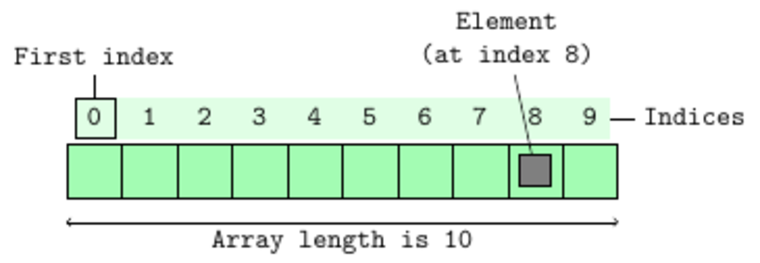
\includegraphics[width=0.7\linewidth]{images/array.pdf}
	\caption{Array}
\end{figure}

\section{Linked List}
\begin{itemize}
	\item Die Linked List ist eine einfach verkettete Liste. Man hat also immer nur Zugriff auf das nächste Element
	\item Jeder Knoten besitzt ein Element (das effektive Objekt) und einen Link zum nächsten Knoten
	\item Dynamische Grösse
	\item Kein umkopieren beim Hinzufügen und Entfernen
	\item Allozierter Speicher entspricht genau den Nutzdaten
	\item Zugriff auf das letzte rsp. mittlere (bei Doubly Linked List) sehr langsam $\Rightarrow$ $\mathcal{O}(n)$
	\item Jeder Knoten besteht aus einem Pärchen bestehend aus dem Element und dem Link zum nächsten Knoten.
	\item Start und Ende der Linked List ist speziell gekennzeichnet. Die leere Linked List hat also mindestens zwei Elemente (Header und Trailer Node). 
	\item Die Java Implementierung der Linked List ist eine Doubly Circular Linked List (wegen dem Deque Interface)
\end{itemize}

\begin{lstlisting}
// Durch alle Elemente loopen
for (Element e = header.next; e != trailer; e = e.next)
\end{lstlisting}

\begin{figure}[h!]
	\centering
	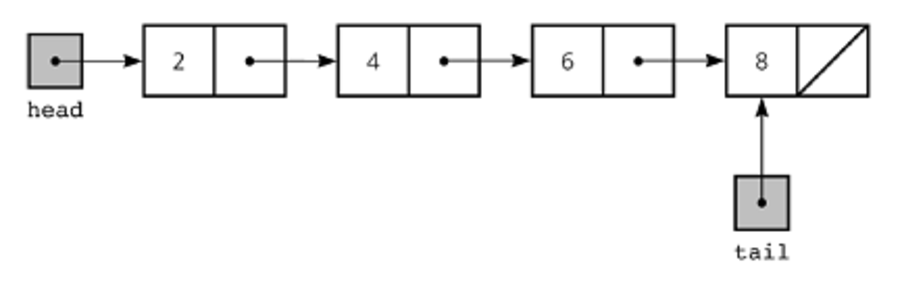
\includegraphics[width=0.5\linewidth]{images/linked_list}
	\caption{Linked List}
\end{figure}

\subsection{Singly Linked List}
\begin{itemize}
	\item Beim Einfügen am Anfang einer Singly Linked List verweist das neue Element auf den aktuellen Head. Zusätzlich wird das Head Flag beim neuen Element gesetzt und beim alten Head entfernt.
	\item Beim Einfügen am Ende einer Singly Linked List verweist das neue Element auf null und das alte Tail verweist auf das neue Element. Zusätzlich wird das Tail Flag beim neuen Element gesetzt und beim alten Tail entfernt.
	\item Singly Linked Lists haben den Nachteil, dass man immer von vorne nach hinten durch iterieren muss. $\mathcal{O}(n)$
\end{itemize}

\subsection{Doubly Linked List}
\begin{itemize}
	\item Jeder Knoten besteht aus einem Triple, bestehend aus dem Element (Wert) und einem Link nach vorne einen nach hinten. (prev, next)
	\item Die leere Liste hat mindestens zwei Knoten (Head, Tail). Head und Tail müssen im Konstruktor verbunden werden.  (next, prev)
\end{itemize}

\begin{figure}[h]
	\centering
	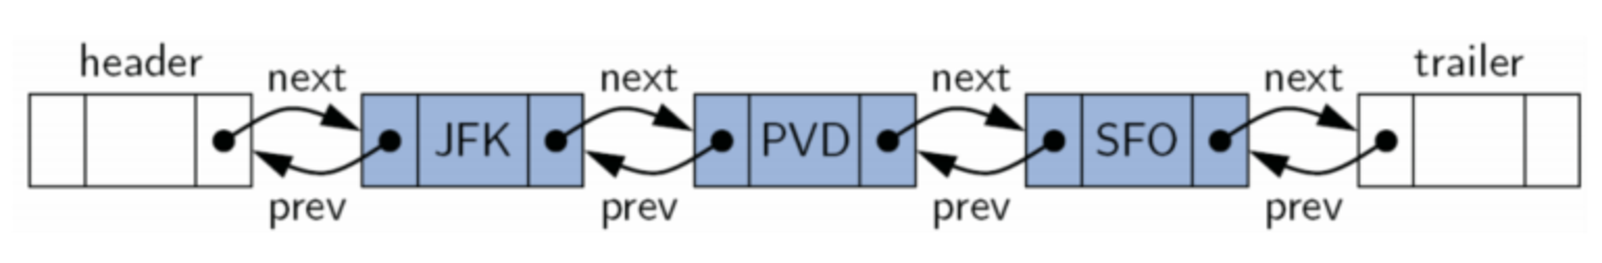
\includegraphics[width=0.5\linewidth]{images/doubly_linked_list}
	\caption{Doubly Linked List / Doppelt verkettete Liste}
\end{figure}

\subsection{Circularly Linked List}
Bei einer Circulary Linked List ist das Tail mit dem Head verbunden

\section{Lists}

\begin{lstlisting}
public interface List<E> {
	size();
	
	boolean isEmpty();
	
	// Gibt das Element an der Stelle i zurueck ohne es zu entfernen
	E get(int i);

	// Fuegt ein Element an der Stelle i in die Liste ein und verschiebt alle nachfolgenden Elemente um eine Stelle
	void add(int i, E element)
	
	// Ersetzt das Element beim Index i und liefert das alte Element zurueck
	void set(int i, E element);	
		
	// Entfernt das Element an der Stelle i und gibt es zurueck
	E remove(int i);
}
\end{lstlisting}

\subsection{ArrayList}
\begin{itemize}
	\item Die Klasse ArrayList speichert die Daten intern in einem primitiven Array
	\item Die Arraylist hat eine variable Grösse und vergrössert das interne Array (fixe Grösse) selbständig
	\item Der Zugriff mit get(), set(), size(), isEmpty() ist $\mathcal{O}(1)$
	\item Beim Einfügen und Entfernen muss immer Platz geschaffen/entfernt werden. (add(i, e), remove(i)) Im schlimmsten Fall müssen alle Elemente verschoben werden $\Rightarrow$ $\mathcal{O}(n)$. Der absolute Worst Case ist i=0, dann dann alle n Elemente verschoben werden müssen.
\end{itemize}

\subsubsection{Strategien dynamische Arraygrösse}
Es gibt zwei Ansätze wie das interne Array vergrössert wird:
\begin{enumerate}
	\item Inkrementelle Strategie: Erweitern der Grösse um eine Konstante k  $\Rightarrow \mathcal{O}(n^2)$
	\item Verdoppelung Strategie: Verdoppeln der Arraygrösse $\Rightarrow \mathcal{O}(n)$
\end{enumerate}

\subsection{Positional-List / Node-List}
\begin{itemize}
	\item Jeder Knoten besitzt einen Vorgänger und einen Nachfahren. Dies erlaubt es Beziehungen zwischen den Knoten zu ziehen. (Ausnahme: Head und Tail)
	\item Jeder Knoten ist ein Position Objekt, welches eine Referenz auf das Element hält.
	\item Benötigt für eine List mit n Elementen $\mathcal{O}(n)$ Speicher
	\item Alle Operationen des Node-List ADT benötigt $\mathcal{O}(1)$ Zeit, sofern man sich an der Position p befindet. 
	\item Die Operation getElement() benötigt $\mathcal{O}(1)$
	\item Suche nach einer Position benötigt $\mathcal{O}(n)$
	\item Eine Doubly Linked List stellt eine einfache Implementierung des Positional List ADT dar.
\end{itemize}
\begin{figure}[h!]
	\centering
	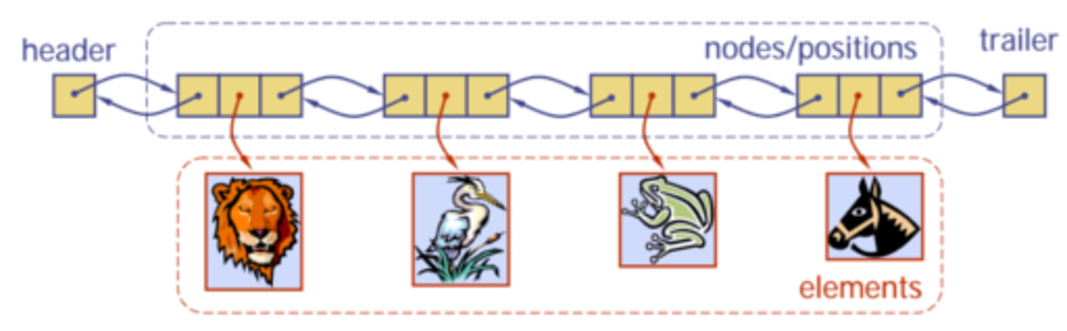
\includegraphics[width=0.7\linewidth]{images/positional_list}
	\caption{Positional List}
\end{figure}
\begin{lstlisting}
public interface Position<T> {
	Position<T> first();
	Position<T> last();
	
	Position<T> addFirst(T element);
	Position<T> addLast(T element);
	
	// Gibt die Position vor oder nach der gegeben Position zurueck
	Position<T> before(Position<T> position);
	Position<T> after(Position<T> position);
	
	// Setzt die Position vor oder nach der gegeben Position
	Position<T> addBefore(Position<T> p, T e) throws IllegalArgumentException;
	Position<T> addAfter(Position<T> p, T e)throws IllegalArgumentException;
	
	E set(Position<T> p, T e) throws IllegalArgumentException;
	E remove(Position<T> p) throws IllegalArgumentException;
	
	Iterator<T> iterator();<
	Iterable<Position<T>> positions();
}
\end{lstlisting}


\subsection{Skip List}
\begin{itemize}
	\item Eine Skip Liste besteht aus einer Menge von Sub Listen
	\item jede Subliste ist sortiert
	\item die Enden jeder Subliste ist mit eindeutigen Sentinels markiert. Gibt es mehrere 'leere' Sublisten mit zwei Sentinels werden alles bis auf einen gelöscht.
	\item Ist besonders geeignet für Multithreading
	\item In einer perfekten Skip Liste ist die Höhe = $log_2(n)$
	\item Jeder $2^k$ Knoten hat einen Zeiger auf den $2^k$ entfernten Knoten auf Niveau k
	\item Beim Einfügen wird mit einer Wahrscheinlichkeit von 50\% entschieden ob der Turm erhöht wird oder nicht.
	\item Der Suchpfad wird in einer temporären Liste abgespeichert
	\item Suchen, Einfügen und Löschen läuft mit $\mathcal{O}$(log(n))
\end{itemize}
\begin{figure}[h]
	\centering
	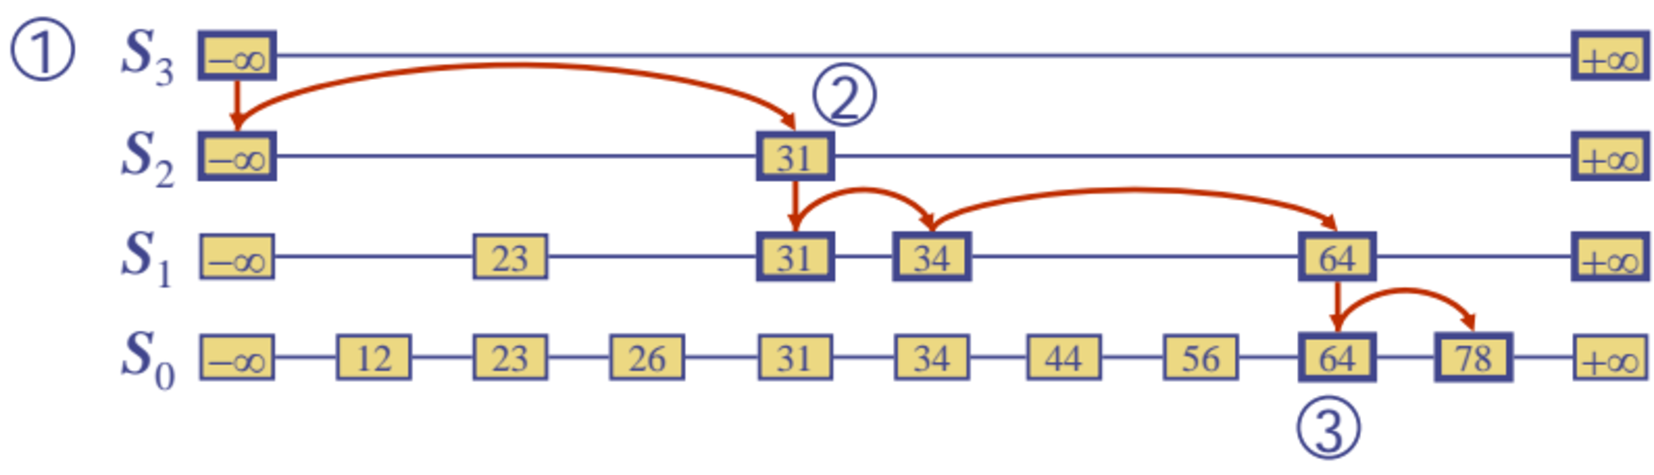
\includegraphics[width=0.8\linewidth]{images/skip_list}
	\caption{Skip List}
\end{figure}

\subsubsection{Vorgehen Einfügen}
Die Elemente einer Skipliste werden mit der Hilfe einer Zufallssequenz eingefügt. (50\% Chance für Inkrementierung der Ebene)
\begin{enumerate}
	\item Erstes Element aus der Liste entnehmen und in Level $S_0$ eintragen. Die Elemente werden auf der x-Achse nach ihren Werten geordnet (links=$-\infty$ und rechts=$+\infty$)
	\item Aus der Zufallssequenz nächste Zahl entnehmen und durchstreichen
	\begin{enumerate}
		\item 1 (Kopf) $\Rightarrow$ Turm erhöhen mit aktuellem Element
		\item 0 (Zahl) $\Rightarrow$ nächstes Element aus der Liste nehmen und auf Level $S_0$ einfügen.
	\end{enumerate}
\end{enumerate}

\subsubsection{Vorgehen Suche}
\begin{enumerate}
	\item Wenn das gesuchte Objekt grösser oder gleich dem \underline{nächsten Objekt} ist, wird scanForward() ausgeführt. Die Operation ''scanForward'' iteriert auf der aktuellen Liste nach vorne. Falls scanForward() $+\infty$ zurückgibt wird dropDown() ausgeführt.
	\item Wenn das gesuchte Objekt grösser oder gleich dem \underline{aktuellen Objekt} ist, wird dropDown() ausgeführt. Die Operation ''dropDown'' geht eine Ebene tiefer.
	\item Falls man auf der untersten Ebenen angelangt ist und ein weiteres Mal dropDown() ausgeführt wird, muss null zurückgegeben werden.
\end{enumerate}

\section{Sets}
\begin{itemize}
	\item Enthält nie Duplikate
	\item Ist unsortiert
\end{itemize}

\begin{lstlisting}
public interface Set<E> {
	add(e)
	remove(e)
	contains(e)
	iterator();
	addAll();
	retainAll();
	removeAll();
}
\end{lstlisting}

\subsection{Multiset}
\begin{itemize}
	\item Erlaubt Duplikate
\end{itemize}

\section{Maps}
\begin{itemize}
	\item Eine Map ist eine durchsuchbare Struktur von Key-Value-Entries.
	\item Pro Key ist nur ein Entry erlaubt!
\end{itemize}


\begin{lstlisting}
public interface Map<K,V> {
	// Gibt Value oder null fuer den Key k zurueck
	get(k);
	// Ersetzt den Wert fuer den Key k. Falls kein Entry fuer k existiert wird ein neues Angelegt und null zurueckgegeben. Ansonsten wird das ersetzte letzte Wert retourniert
	put(k, v);
	// Gibt den Wert fuer k zurueck und loescht das Entry in der Map. Gibt es keinen Eintrag fuer k wird null zurueckgegeben.
	remove(k);
	// Liefert iterierbare Collection aller Schluessel
	keySet();
	// Liefert iterierbare Collection aller Werte
	values();
	// Liefert iterierbare Collection aller Eintraege
	entrySet();
}
\end{lstlisting}

\subsection{Map als List}
Eine Map kann ganz einfach mit einer doppelt verketten Liste implementiert werden. Dieser Ansatz ist jedoch nur bei kleinen Maps sinnvoll, da die Funktionen put(), get() und remove() mit $\mathcal{O}(n)$ laufen. $\mathcal{O}(n)$ daher, da die ganze Liste auf Duplikate durchsucht werden muss. Dabei wird die Key-Value Entries als Elemente der Liste abgespeichert.

\paragraph{Sentinel Trick}
Der gesuchte Knoten wird in einem ersten Schritt als Trailer der List hinzugefügt. Danach kann man über die Liste iterieren ohne immer prüfen zu müssen, ob man das Ende der Liste erreicht hat.
\begin{lstlisting}
private MapEntry<K, V> find(Object key) {
	MapEntry<K, V> sentinel = new MapEntry<K, V>((K)key, null);
	list.addLast(sentinel); 
	Iterator<MapEntry<K, V>> it = list.iterator();
	while (true) {
		MapEntry<K, V> e = it.next();
		K thisKey = e.getKey();
		if (thisKey.equals(key) || thisKey != null && thisKey.equals(key)) {
			list.removeLast();  // remove sentinel
			if (e.equals(sentinel)) {
				return null;
			} else {
				return e;
			}
		}
	}
}
\end{lstlisting}

\subsection{Hashtabelle}
Eine Hashtabelle besteht immer aus den folgenden zwei Elementen
\begin{enumerate}
	\item Einer Hashfunktion wessen resultierender Hashwert als Index für das Array verwendet wird.
	\item Einem Array mit einer fixen Grösse 
\end{enumerate}

\subsection{HashMap}
Bei einer HashMap werden die Keys mit einer Hashfunktion gehashed. Die resultierenden Hashwerte dienen als Index in dem dahinter liegenden Array. Eine gute Hashfunktion verteilt die Einträge so gut, dass keine Kollisionen auftreten. (gute Streuung) Wenn der generierte Hashcode grösser wie der grösste Index des Arrays ist, wird der Hashcode modulo Array Länge gerechnet. (Kompressionsfunktion) Gibt es eine Kollision (zwei Einträge auf einem Index) wird eine verkettete Liste an der Position des Indexes angelegt. 

\subsection{Kompressionsfunktion}
\begin{itemize}
	\item Als Grösse für die Hashtabelle wird aufgrund der Zahlentheorie oft eine Primzahl verwendet.
	\item Zur Kompression wird meist der resultierende Hashwert modulo Hashtabellengrösse verwendet.
\end{itemize}

\subsection{Kollisionsbehandlung}
\begin{description}
	\item[geschlossene Adressierung] \hfill \\ Bei einer Kollision werden weitere Objekte in einer verketteten Liste abgelegt. Diese Variante erfordert eine weitere Datenstruktur, was zusätzlicher Speicherverbrauch bedeutet.
	\item[offene Adressierung] \hfill \\ Bei einer Kollision wird einfach der nächste offene Platz gesucht. Dabei gibt es diverse Varianten wie die ''nächste'' offene Stelle gesucht wird. (linear nach vorne, linear nach hinten, (linear Probing) quatrischer Ansatz, etc.)
	\item[Doppeltes Hashing] \hfill \\
	Hierbei wird bei einer Kollision einen zweiten Hashwert berechnet. Das Resultat des zweiten Hashwertes entspricht dann den Anzahl Stellen um welche verschoben wird. $Hashwert = (h_1(k) + c\cdot h_2(k)) mod N$ (c = Anzahl Kollisionen)
\end{description}

\subsubsection{Löschen bei linearer Sondierung}
Soll ein Datensatz gelöscht werden, so kann dies die Sondierungsfolge für einen andere Datensatz unterbrechen. Deshalb darf man die Einträge nicht wirklich löschen sondern nur als gelöscht markieren. $\Rightarrow$ Spezielles Dummy Objekt ablegen. (DEFUNCT Objekt)

\subsection{Polynom Akkumulation / Horner Schema}
Man zerlege die Bits eines Schlüsseles in mehrere Teile fixer Länge und berechne davon das Polynom $p(z) = a_0 + a_1 z + a_2 z + ... + a_{n-1}z^{n-1}$. Das Polynom p(z) kann in $\mathcal{O}(n)$ mithilfe des Horner Schemas berechnet werden. Dieses Verfahren wird von Java verwendet.

\subsubsection{String Hashcode}
Der Hashcode für String wird unter Java wie folgt berechnet
\[
hashcode = stringArr[0] \cdot 31^{n-1} + stringArr[1] \cdot 31^{n-2} + ... + stringArr[n-1]
\]

\subsection{Performance}
Hashing ist grundsätzlich sehr schnell ist im Idealfall $\mathcal{O}(1)$ wenn keine Kollisionen auftreten. Ansonsten kann das Laufzeitverhalten zu $\mathcal{O}(n)$ führen.

\subsection{Multimap / Dictionary}
\begin{itemize}
	\item Pro Key gibt es mehrere Werte
	\item Auch bekannt als Dictionary
	\item Es gibt zwei Ansätze wie eine Multimap implementiert werden kann
	\begin{enumerate}
		\item Ein Schlüssel verweisst auf eine Collection mit Werten zu einem Key
		\item Anpassen der darunterliegenden Datenstruktur, das mehrere Key gespeichert werden können
	\end{enumerate}
\end{itemize}

\section{Queues}
\begin{itemize}
	\item Eine einfache Queue ist FIFO. 
	\item Das Einfügen erfolgt am Ende der Queue, das Entfernen am Anfang
	\item z.B Round Robin Scheduler
\end{itemize}

\begin{lstlisting}
public interface Queue<E> {

public int size();

public boolean isEmpty();

// Fuegt ein Element am Ende der Queue ein
public void enqueue(E element);

// Entfernt und gibt das Element am Anfang der Queue zurueck.
public E dequeue();

// Liefert das erste Element ohne es zu entfernen
public E first();
}
\end{lstlisting}

\subsection{Ringer Buffer / Array basierte Queue}
Queues sind häufig als Ringpuffer mit je einem Zeiger auf Anfang (In-Pointer) und Ende (Out-Pointer) implementiert. Die Besonderheit des Ringpuffers ist, dass er eine feste Größe besitzt. Dabei zeigt der In-Pointer auf das erste freie Element im Array, das den Ringpuffer repräsentiert, und der Out-Pointer auf das erste belegte Element in dem Array. Im Unterschied zum Array werden die ältesten Inhalte überschrieben, wenn der Puffer voll ist und weitere Elemente in den Ringpuffer abgelegt werden.


\[
Index_{rear} = (Index_{front} + Number_{elements} \text{ mod }(Array_{length})) 	
\]

\subsection{Listen Basierte Queue / Node Queue}
\begin{lstlisting}
Node<E> head;
Node<E> tail;
int numberOfElements;
\end{lstlisting}

\subsection{Double Ended Queue / Deque}
\begin{itemize}
	\item Bidirektionale Queue
	\item Das Einfügen und Entfernen erfolgt am Anfang oder am Ende
	\item Wird am einfachsten intern mit einer Doubly Linked List implementiert
\end{itemize}
\begin{lstlisting}
addFirst(Element e); 
addLast(Element e);
Element removeFirst(); 
Element removeLast();
\end{lstlisting}

\begin{figure}[h]
	\centering
	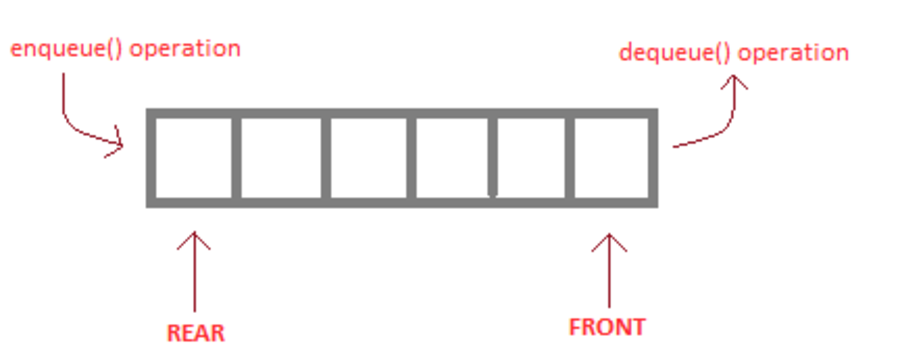
\includegraphics[width=0.7\linewidth]{images/queue.pdf}
	\caption{Queue}
\end{figure}

\subsection{Priority Queues}
\begin{itemize}
	\item Eine sortierte Queue
	\item Eine Priority Queue ist eine Collection aus Entries, bestehend aus Key Value Paaren.
	\item Die interne Datenstruktur ist nach dem Key der Entries geordnet
	\item Mittels removeMin() können die Elemente sortiert entfernt werden.
	\item Mithilfe der Priority Queue kann ein Set aus vergleichbaren Elementen sortiert werden.
	\begin{description}
		\item[Selection Sort] Schnelles Einfügen ($\mathcal{O}(1)$), langsames herausnehmen, da die Werte beim Herausnehmen sortiert werden. ($\mathcal{O}(n)$)
		\item[Insertion Sort] Langsames einfügen ($\mathcal{O}(n)$), schnelles herausnehmen ($\mathcal{O}(1)$), da die Werte beim Einfügen sortiert werden.
		\item[In-Place Implementierung] Bei einem In-Place Algorithmus wird keine zusätzliche Datenstruktur verwendet, als jede die für die Speicherung der Daten benötigt wird. 
	\end{description}
\end{itemize}

\begin{lstlisting}
//fuegt ein Entry mit Schluessel k und Wert v ein
insert(k,v);
// entfernt und liefert die Entry mit dem kleinsten Schluessel
removeMin();
// gibt die Entry mit dem kleinsten Schluessel zurueck ohne diese zu entfernen
min();
size();
isEmpty();
\end{lstlisting}

\subsection{Adaptierbare Priority Queue} 
\begin{itemize}
	\item Bei einer normalen Priority Queue kann ein beliebiger Node nicht einfach geändert werden. Man müsst dazu alle Nodes bis zum gesuchten Node entfernen
	\item Die adaptierbare PQ implementiert deshalb drei weitere Methoden:
	\begin{lstlisting}
	// Entfernt das Element und gibt es zurueck
	remove(e);
	// Der Schluessel des Element e wird durch k ersetzt
	replaceKey(e, k);
	// Der Wert des Elements e wird durch v ersetzt
	replaceValue(e, v);
	\end{lstlisting}
	\item Eine Location Aware Entry weiss über seine Position innerhalb der Datenstruktur bescheid. Dazu hat jedes Knotenelement eine Rückreferenz auf den Knoten
	\item Die Listen basierte Implementierung verwendet dabei eine Positional List
	\item Bei der Heap Implementierung zeigt jeder Knoten auf das Werte Objekt und dieses hat wiederum eine Back Reference auf den Knoten. Der Back Pointer müssen bei up-, und downheaps() aktualisiert werden und sind deshalb optional.
\end{itemize}

\section{Stack}
\begin{itemize}
	\item LIFO Prinzip: Das zuletzt eingefügte Element wird zuerst herausgenommen.
	\item Man hat immer nur auf das oberste Element Zugriff
	\item Die JVM ist eine Stack Maschiene. Sie speichert aktive Methoden in der Reihenfolge ihres Aufrufs auf dem Stack.
\end{itemize}

\begin{lstlisting}
public interface Stack<E> {

	public boolean empty();
	
	// Top des Stacks ohne entfernen des obersten Elements
	public E top();
	public E peek(); // Java Util
	
	// Entfernt das oberste Element
	public E pop();
	
	// Legt ein Element zuoberst auf den Stack
	public void push(E elem);
}
\end{lstlisting}

\begin{figure}[h]
	\centering
	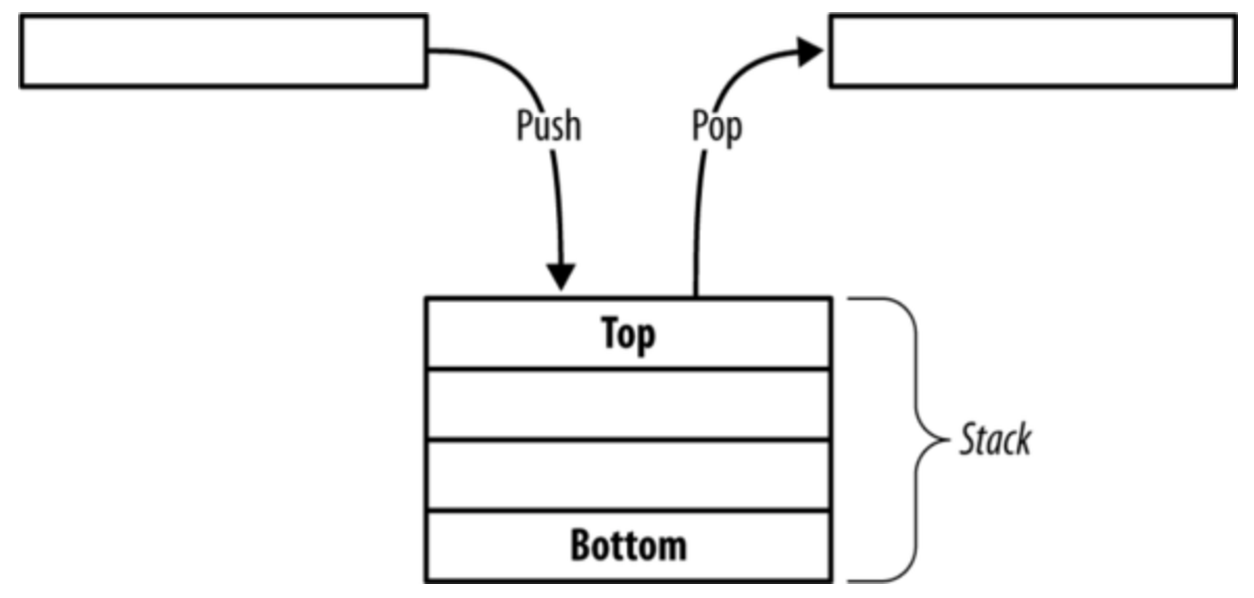
\includegraphics[width=0.5\linewidth]{images/stack.pdf}
	\caption{Stack}
\end{figure}

\subsection{Array basierter Stack}
\begin{itemize}
	\item Jede Operation läuft mit $\mathcal{O}(1)$
	\item Es wird eine zusätzliche Variable für den Top of Stack benötigt
	\item Die maximale Grösse des Arrays ist fix. Der Stack muss bei bedarf erweitert und verkleinert werden.
\end{itemize}

\subsection{Listen basierter Stack}
\begin{itemize}
	\item top() $\Rightarrow$ first();
	\item push() $\Rightarrow$ addFirst(e);
	\item pop() $\Rightarrow$ removeFirst();
\end{itemize}

\section{Tree}
\begin{itemize}
	\item Hierarchische Struktur wobei die Wurzel zuoberst ist
	\item Es gibt eine Eltern Kind Relation zwischen zwei Knoten
\end{itemize}

\begin{description}
	\item[k-Baum] Ein Baum mit k Kindknoten pro Node
	\item[Wurzel / Root] Elternknoten
	\item[Interner Knoten] Knoten mit min. einem Child
	\begin{lstlisting}
	public computeInternNodes(Node<T> root) {
		if (root == null || root.left == null && root.right == null) {
			return 0;
		} else {
			return 1 + computeInternNodes(root.left) + frage(root.right);
		}
	}
	\end{lstlisting}
	\item[Externer Knoten / Blattknoten] Knoten ohne Childs: 
	\[
		Anz_{\text{externe Knoten}} = Anz_{\text{interne Knoten}} \cdot (Anz_{\text{Kind Knoten pro Baum}} -1) + 1
	\]
	\item[Vorgängerknoten] Parent
	\item[Tiefe] Anzahl Vorgänger (nach oben)
	\begin{itemize}
		\item Wenn Wurzel Knoten: Tiefe = 0
		\item Ansonsten: Hole rekursiv die Tiefe des Parents und zähle 1 dazu
	\end{itemize}
	\item[Höhe] Anzahl Ebenen der Nachfolger (nach unten). Die Höhe gibt die Anzahl Ebenen des Baumes an.
	\begin{itemize}
		\item Externe Knoten haben die Höhe 0
		\item Hole rekursiv die maximale Höhe aller Children und zähle 1 dazu
	\end{itemize}
	\item[Subtree] Baum aus einem Knoten und seinen Nachfolger
	\item[Vorgängerknoten] Parent
	\item[Siblings] Zwillingsknoten
\end{description}

\begin{lstlisting}
public interface Tree {
	// Zugriffsmethoden
	Position<E> root()
	Position<E> parent(Position<E> p)
	PositionList<E> children(Position<E> p)

	//Abfragemethoden
	int numChildren(Position<E> p) // nur die direkten Kinder! (Eine Ebene tiefer)
	boolean isInternal(Position<E> p) // mit child
	boolean isExternal(Position<E> p) // ohne child
	boolean isRoot(Position<E> p)
	
	//Hilfsmethoden
	int size();
	boolean isEmpty();
	int iterator();
	PositionList<E> positions();
}
\end{lstlisting}

\subsection{Speicherverfahren}
\subsubsection{Linked List}
Jeder Knoten wird von einer Klasse representiert die aus den folgenden drei Elementen besteht:
\begin{itemize}
	\item Eine Referenz auf den Knoten Wert
	\item Eine Referenz auf den Parent Knoten
	\item Eine Referenz auf auf eine List von Child Knoten. Wenn es sich um einen Binary Tree handelt, wird auf die Liste verzichtet. Stattdessen wird die Referenz auf den linken und rechten Knoten direkt gespeichert.
\end{itemize}

\subsubsection{Array}
Das folgende Konzept funktioniert nur für den Binärbaum
\begin{enumerate}
	\item Der Root Knoten kommt auf den Index 1
	\item Der Linke Kind Knoten kommt auf den Index: $2 \cdot Index_{parent}$
	\item Der Rechte Kind Knoten kommt auf den Index: $2 \cdot Index_{parent} + 1$
\end{enumerate}

\subsection{Traversierung}
Gestartet wird immer beim Root, aufgeschrieben wird aber nur gemäss der Euler Tour Traversierung. Dabei zeichnet man startend links vom Parent Node eine Umrandung um den ganzen Tree und zieht bei jedem Knoten einen Strich in eine bestimmte Richtung:
\begin{description}
	\item[Preorder / Strich nach Links] Ein Node wird vor seinen Nachfolgern besucht, wobei zuerst der linke Node und danach der rechte Node abgearbeitet wird. ($Parent Node \Rightarrow Left Node \Rightarrow Right Node$)
	\item[Postorder / Strich nach Rechts] Ein Node wird nach seinen Nachfolgern besucht ($Left Node \Rightarrow Right Node \Rightarrow Parent Node$). Diese Variante kann für das berechnen von arithmetischen Audrücken verwendet werden.
	\begin{lstlisting}
	calcRecursive(n) {
		if (isExternal(n)) {
			return n.element();
		} else {
			x = calcRecursive(leftChild(n));
			y = calcRecursive(rightChild(n));
			o = parseOperator(v);
			return x o y;
		}
	}
	\end{lstlisting}
	\item[Inorder / Strich nach Unten] Ein Knoten wird \textbf{nach} seinem linken Subtree und \textbf{vor} seinem rechten Subtree besucht.
	($Left Node \Rightarrow Parent Node \Rightarrow Right Node$) Diese Variante kann für das ausgeben von arithmetischen Ausdrücken verwendet werden.
	\begin{lstlisting}
	printExpression(n) {
	if (hasLeft(n)) {
		print('(');
		printExpression(left(n));
	}
	print(n.element());
	if (hasRight(n)) {
		printExpression(right(n));
		print(')');
	}
	\end{lstlisting}
	\item[Breath First / Level Traversierung] Es werden zuerst alle Nodes einer Ebenen besucht bevor man zu einer tieferen Ebenen voranschreitet. Die Nodes werden dabei von links nach rechts abgearbeitet.
	\begin{lstlisting}
	Queue<TreeNode> queue = new LinkedList<BinaryTree.TreeNode>() ;
		public void breadth(TreeNode root) {
			if (root == null)
				return;
			queue.clear();
			queue.add(root);
			while(!queue.isEmpty()){
				TreeNode node = queue.remove();
				System.out.print(node.element + " ");
				if(node.left != null) queue.add(node.left);
				if(node.right != null) queue.add(node.right);
		}
	}
	\end{lstlisting}
	
\end{description}

\subsection{Binärbaum}
\begin{description}
	\item[Vollständiger Binärbaum] \hfill \\
	Bei einem vollständigen Binärbaum sind alle Level bis auf das letzte vollständig aufgefüllt. Zusätzlich muss das letzte Level von links nach rechts aufgefüllt sein. Es gibt maximal ein Knoten mit nur einem Kind, welcher ein linker Knoten sein muss.
	\item[Echter Binärbaum (full/proper)] \hfill \\
	Jeder interne Knoten besitzt genau zwei Kindknoten
	\item[Balancierter Baum] \hfill \\ 
	Bei einem Balancierten Baum haben alle Subtrees auf jeder Ebene die selbe Höhe
\end{description}
\begin{itemize}
	\item Die Position eines einmal eingefügten Knotens wird nicht mehr verändert
	\item Jeder interne Knoten besitzt höchstens zwei Kinder. Bei echten Binärbäumen müssen es immer genau zwei Kindknoten sein
	\item Die Kinder eines Knoten sind ein geordnetes Paar (links, rechts $\Rightarrow$ sortiert). Die Ordnung ist dabei Definitionssache
	\item Jeder Subtree ist wiederum ein Binärbaum
	\item Anwendungsfälle sind:
	\begin{itemize}
		\item Arithmetische Ausdrücke: Jeder Subtree stellt ein Klammerausdruck dar, wobei der Parent die Operation und die beiden Kinder die Zahlen/Variablen representieren.
		\item Entscheidungsprozesse: Jeweils links oder auch rechts ist immer die selbe Entscheidung.
		\item Binäre Suche
	\end{itemize}
\end{itemize}
\begin{lstlisting}
public interface BinaryTree<E> extends Tree<E> {
	// Ein Binaerbaum besitzt zusaetzliche Methoden
	Position<E> left(Position<E> p);
	Position<E> right(Position<E> p);
	Position<E> sibling(Position<E> p);
}
\end{lstlisting}

\subsection{Postorder Calculator}
Die Umgekehrt Polnische Notation verwendet Postorder Calculation nach folgendem Prinzip:
\begin{algorithm}
\begin{algorithmic}[1]
	\IF{$isExternal(v)$} 
		\RETURN{$v.element()$} 
	\ELSE
		\STATE $ x \gets  evalExpr(leftChild(v))$
		\STATE $ y \gets  evalExpr(rightChild(v))$
		\STATE $ o \gets  $ Operator bei v
		\RETURN $x parse(o) y$
	\ENDIF
\end{algorithmic}
\caption{evalExpr(v)}
\end{algorithm}

\section{Heaps}
Ein Heap ist ein vollständiger Binärbaum (von links her aufgefüllt), der in seinen Knoten Schlüssel speichert, wobei jeder Kindknoten einen grösseren oder gleichen Key als sein Parent haben muss. Das kleinste Element ist somit immer der Root-Knoten. Ist gibt auch sogennante MAX-Heaps wobei der Root Knoten das grösste Element ist.

\begin{figure}[h!]
\centering
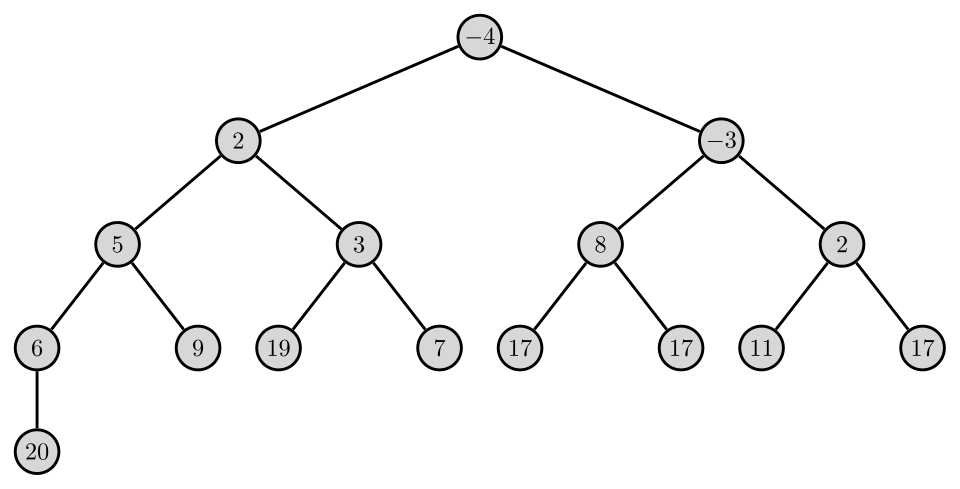
\includegraphics[width=0.5\linewidth]{images/heap}
\caption{MAX-Heap in Baum und Array Ansicht}
\end{figure}


\subsection{Heaps als Priority Queue}
\begin{itemize}
	\item Jeder Knoten ist ein paar aus Key-Value
	\item Der letzte Knoten wird speziell markiert
	\item Neue Knoten werden immer nach dem letzten Knoten eingefügt
	\item Solange der neue Knoten kleiner wie sein Parent ist, switched die Funktion upheap() der Parent und den Child
	\item Die Funktion upheap läuft mit $\mathcal{O}$(log n), da sie von der Höhe abhängt. 
	\item Die Höhe ist ebenfalls $\mathcal{O}$(log n)
	\item Mit der Methode removeMin() kann das kleinste Element entfernt werden. Dies ist immer der Root Knoten
	\begin{itemize}
		\item Zuerst wird der Root Knoten entfernt und mit dem letzten Knoten ersetzt
		\item Danach wird der letzte Knoten gelöscht
		\item Schliesslich stellt die Methode downHeap die Ordnung wieder her, indem die Knoten von oben nach unten gemäss ihrer Grösse vertauscht werden.
	\end{itemize}
	\item Die Methode downHeap() läuft mit $\mathcal{O}$(log n)
	\item Der Heap muss von oben nach unten und von links nach rechts immer sortiert sein. Der Grösste Key ist immer ganz unten links!
\end{itemize}

\subsection{Heap Sort / Bottom Up Konstruktion}
\begin{itemize}
	\item Läuft mit $\mathcal{O}$(n log n)
	\item Beim Heap Sort wird die Bottom Up Kontruktion verwendet. Der Heap wird also von unten nach oben aufgebaut. Dabei werden immer zwei Teilheaps (mit $2^i - 1$ Elementen $\Rightarrow$ i = Phase) zu einem grösseren Heap (mit $2^{i+1} - 1$ Elementen) zusammengeführt.  $\Rightarrow$ benötigt $\mathcal{O}(n)$ um den Heap Bottom Up aufzubauen
\end{itemize}

\section{Itertor}
Ein Iterator besteht grundlegend aus den beiden Methoden next() und hasNext()
\begin{lstlisting}
// Prueft ob es ein naechstes Element gibt (Cursor). Zeigt immer zwischen zwei Elemente
hasNext();
// Gibt das naechste Element in der Liste zurueck
next();

// Nur fuer Doubly Linked List Iteratoren
hasPrevious()
previous()
\end{lstlisting}


Es gibt zwei grundlegende Varianten
\subsection{Snapshot Iterator}
Es wird eine Kopie der Ausgangsdatenstruktur genommen. Änderungen auf beeinflussen die Ausgangsdatenstruktur nicht. Da zuerst die Datenstruktur kopiert werden muss, läuft diese Variante mit $\mathcal{O}(n)$. 

\subsection{Lazy Iterator}
Dies ist die meist verbreitete Variante wobei die Iterationen auf Original Datenstruktur durchgeführt werden. Strukturänderungen an der Datenstruktur durch einen anderen Prozess können die Iteration verunmöglichen. (ConcurredModificationException) Da nichts umkopiert werden muss, sind die Kosten dafür gering.

\subsection{Iterator vs For-Schleife}
\begin{itemize}
	\item Die Variante mit dem Iterator läuft mit $\mathcal{O}(n)$ da der Iterator die zugrunde liegende Datenstruktur kennt
	\item Die Variante mit einer For Schleife und der get(i) Funktion läuft mit $\mathcal{O}$($n^2$) da bei der Get Funktion noch einmal die ganze Liste bis zum i-ten Element durchlaufen werden muss.
\end{itemize}



\section{Algorithmen}
\subsection{Binäre Suche}
Die binäre Suche verwendet den Divide and Conquer Algorithmus
\begin{lstlisting}
public boolean binarySearch(int[] data, int taget, int low, int high) {
	if (low > high) 
		return null;
	} else {
		int mid = (low + high) / 2;
		if (target == data[mid]) {
			// Hit
			return true;
		} else if (target < data[mid]) {
			return binarySearch(data, target, low, mid -1);
		} else {
			return binarySearch(data, target, mid + 1, high);
		}
	}
}
\end{lstlisting}


\paragraph{Doubly Linked List basierter Ansatz} \hfill \\
\begin{lstlisting}
public Integer binarySearch(Integer key) {
	Node node = head;
	// amount of compareTo() used for direction
	int compare = 1; 
	// Empty list = 0
	int len = (noOfNodes + 1);
	while (len > 0) {
		len = len / 2;
		if (len == 0) {
			i = -1;
			for (; i < len; i++) {
				if (compare > 0) {
					node = node.next();
				} else {
					node = node.prev();
				}
			}
			if ((node == head) || (node == tail)) {
				return null;
			}
			compare = key.compareTo(node.key);
			if (compare == 0) {
				return node.value;
			}
		}
		return null;
	}	
}
\end{lstlisting}

\subsection{Rekursives Array umdrehen}
Dieser Algorithmus ist ein Beispiel für eine Tail Recursion. Das Resultat liegt nach dem Erreichen des Base Cases vor.
\begin{lstlisting}
public class ReverseArray {
  public int[] reverseArray(int[] a, int i, int j) {
	  int temp=a[j];
	  a[j] = a[i];
	  a[i] = temp;
	  reverseArray(a, i+ 1, j - 1);
  }
}
\end{lstlisting}

\subsection{Rekursives Ausgeben einer Linked List} 
\begin{lstlisting}
public static void printReverse(Node<String> head) {
	if (head.next == null) {
		System.out.println(head.element);
	} else {
		// Beachte ob zuerst ausgegeben werden soll und dann rekursiver Aufruf oder umgekehrt
		printReverse(head.next);
		System.out.println(head.element);
	}
}
\end{lstlisting}



\subsection{Rekursives Divide \& Conquer}
Nachdem das Maximum der linken Hälfte bestimmt wurde, wird mit der rechten Hälfte entsprechend weiterverfahren.
\begin{lstlisting}
public char maximum(char[] w, int start, int end) {
	if(start==end) {
		return w[start];
	}
	
	int middle = (start + end) / 2;
	char max1 = maximum(w, s, middle);
	char max2 = maximum(w, middle + 1, end);
	
	if(max1 < max2) {
		return max2;
	}
	return max1;
}
\end{lstlisting}

\subsection{Rekursives Quadrieren}
Die Rekursive Methode läuft mit $\mathcal{O}$(log(n))
\begin{lstlisting}
public double power(double base, int exponent) {
	if (exponent == 0) {
		return 1;
	}
	
	double temp;
	if (exponent % 2 != 0) {
		temp = power(base, (exponent - 1) / 2);
		return base * temp * temp;
	} else {
		temp = power(base, exponent / 2);
		return temp * temp;
	}
}
\end{lstlisting}


\subsection{Klammer Matching}
\begin{lstlisting}
public static boolean parenthesisCheck(String text) {
	Stack<Character> stack = new Stack<>();
	for (int i = 0; i < text.length(); i++) {
		if(text.charAt(i) == '(') {
			stack.push(text.charAt(i));
		} else if (text.charAt(i) == ')') {
	
			// Empty stack or invalid parenthesis
			if (stack.isEmpty() || stack.pop().equals(text.charAt(i))) {
				return false;
			} 
		}
	}

	if (stack.isEmpty()) {
		// all parenthesis matched
		return true;
	} else {
		return false;
	}
}
\end{lstlisting}

\subsection{Insertion Sort}

\paragraph{Array basierter Ansatz} \hfill \\
Beim Insertion Sort wird mit zwei Schleifen gearbeitet. Die äussere started beim Array Index 1 (zweites Objekt) und iteriert über alle Elemente des Arrays. Die innere Schleife nimmt initial den Iteration-Index der äusseren Schleife und vergleicht rückwärts die beiden Elemente auf Unterschiede.
\begin{lstlisting}
public static void InsertionSort( int [] data) {
	for (int i = 1; i < num.length; i++) {    // Start with 1 (not 0)
		int current = data[i];
		int j = i;
		while(j > 0 && data[j - 1] > current) {
			data[j] = data[j - 1];
			j--;
		}
		data[j] = current;
	}
}
\end{lstlisting}

\subsection{Loops in Link List erkennen}
Loops können mit dem ''Floyd's cycle finding algorithm'', welcher auch unter dem Namen ''Tortoise and hare algorithm'' bekannt ist, erkannt werden. Dabei lässt man ein Element doppelt so schnell wie ein anderes durch die Liste gehen. Wenn das schnellere, dass langsamere einholt, gibt es eine Loop.

\begin{lstlisting}
boolean hasLoop(Node first) {
	if(first == null) {
		return false;
	}

	// create two references
	Node slow, fast; 
	
	// make both refer to the start of the list
	slow = fast = first; .

	while(true) {
		// single hop
		slow = slow.next;      
		
		if(fast.next != null) {
			// two hops
			fast = fast.next.next; 
		} else {
			// next node null => no loop.
			return false;          
		}
		// if either hits null..no loop
		if(slow == null || fast == null) {
			return false;
		} 
		// if the two ever meet...we must have a loop
		if(slow == fast) {
			return true;
		}
	}
}
\end{lstlisting}


\section{Datenstrukturen und Algorithmen im Vergleich}
\subsection{Array vs. List}
\begin{itemize}
	\item Array haben schnelleren Zugriff auf den Index i
	\item Listen sind schneller beim Entfernen von Objekten
	\item Arrays sind schneller beim Einfügen an einem bestimmten Index
	\item Listen sind schneller beim Einfügen nach/vor einem bestimmten Objekte
	\item Listen erweitern sich dynamisch. 
	\item Arrays müssen bei add() und remove() erweitert, verkleinert werden
\end{itemize}
\begin{tabu} to \linewidth {|X|X|X|}
	\hline
	Operation & Array & List \\
	\hline \hline
	size(), isEmpty() 	& $\mathcal{O}(1)$ & $\mathcal{O}(1)$ \\ 
	\hline
	atIndex(i), get(i) 	& $\mathcal{O}(1)$ & $\mathcal{O}(n)$ \\
	\hline
	first(), last(), prev(), next() 	& $\mathcal{O}(1)$ & $\mathcal{O}(1)$ \\ 
	\hline
	set(p, e) 	& $\mathcal{O}(1)$ & $\mathcal{O}(1)$ \\
	\hline
	set(i, e) 	& $\mathcal{O}(1)$ & $\mathcal{O}(n)$ \\
	\hline
	add(i, e), remove(i) 	& $\mathcal{O}(n)$ & $\mathcal{O}(n)$ \\
	\hline
	addFirst(e), addLast(e) 	& $\mathcal{O}(n)$ & $\mathcal{O}(1)$ \\
	\hline
	addAfter(p, e), addBefore(p, e) 	& $\mathcal{O}(n)$ & $\mathcal{O}(1)$ \\
	\hline
	remove(p)	& $\mathcal{O}(n)$ & $\mathcal{O}(1)$ \\
	\hline
	indexOf(p) & $\mathcal{O}(n)$ & $\mathcal{O}(n)$ \\
	\hline
\end{tabu}

\subsection{Insertion vs Selection Sort}
\begin{tabu} to \linewidth {|X|X|X|X|}
	\hline
	& Datenstruktur & Best Case & Worst Case \\
	\hline \hline
	Selection Sort & Array & $\mathcal{O}(n^2)$ & $\mathcal{O}(n^2)$ \\ \hline
	Selection Sort & Doubly Linked List & $\mathcal{O}(n^2)$ & $\mathcal{O}(n^2)$ \\ \hline
	Insertion Sort & Array & $\mathcal{O}(n^2)$ & $\mathcal{O}(n^2)$ \\ \hline
	Insertion Sort & Doubly Linked List & $\mathcal{O}(n)$ & $\mathcal{O}(n^2)$ \\ \hline
	\hline
\end{tabu}


\end{document}